\documentclass[11pt,a4paper,ngerman]{article}
\usepackage[bottom=2.5cm,top=2.5cm]{geometry} 
\usepackage{babel}
\usepackage[utf8]{inputenc} 
\usepackage[T1]{fontenc} 
\usepackage{ae} 
\usepackage{amssymb} 
\usepackage{amsmath} 
\usepackage{graphicx}
\usepackage{fancyhdr}
\usepackage{fancyref}
\usepackage{listings}
\usepackage{xcolor}
\usepackage{paralist}

\usepackage[pdftex, bookmarks=false, pdfstartview={FitH}, linkbordercolor=white]{hyperref}
\usepackage{fancyhdr}
\pagestyle{fancy}
\fancyhead[C]{Approximation Algorithms}
\fancyhead[L]{Exercise sheet 1}
\fancyhead[R]{SoSe 2012}
\fancyfoot{}
\fancyfoot[L]{}
\fancyfoot[C]{\thepage \hspace{1px} of \pageref{LastPage}}
\renewcommand{\footrulewidth}{0.5pt}
\renewcommand{\headrulewidth}{0.5pt}
\setlength{\parindent}{0pt} 
\setlength{\headheight}{15pt}

\date{}
\title{Max Wisniewski}
\author{Dozent : Panos Giannopoulos}

\begin{document}

\lstset{language=Pascal, basicstyle=\ttfamily\fontsize{10pt}{10pt}\selectfont\upshape, commentstyle=\rmfamily\slshape, keywordstyle=\rmfamily\bfseries, breaklines=true, frame=single, xleftmargin=3mm, xrightmargin=3mm, tabsize=2}

\renewcommand{\figurename}{Figure}


\maketitle
\thispagestyle{fancy}

%% ------------------------------------------------------
%%                     Exercise 1
%% ------------------------------------------------------

\section*{Exercise 1}

Consider the 2-approximation algorithm for the cardinality (i.e. unweighted) vertex cover problem that is based on computing a maximal matching. What approximation factor does it give for the general weighted vertex cover problem, where the vertices have arbitrary positive weights?\\

\textbf{Solution:}\\
Because $\delta$ is a function which domain is the set of instances for the problem we might take any information from the graph we need. The general idea to estimate the approximation factor is, that on each edge from the maximal matching, there might stand the maximal value of all nodes.\\
Because at least one of these nodes has to be part of the Minimum-Vertex-Cover we consider the worst case. One of these nodes contains the smallest possible value, the other one has the biggest on.\\
Now the weight of the two nodes on the edges we took is $\frac{max+min}{min} = \frac{max}{min}+1$ times as large as the smallest posibility might be.\\
We sum up every node in the maximal matching and because we know we know each pair of the matching is at most $\frac{max}{min}+1$ times as large, we can use the destribution law to extract the factor 
$$
	\delta (G(V,E)) = \frac{\max (V)}{\min (V)} + 1.
$$

\begin{description}
\item{\bfseries proposition} $|C| \leq \left( \frac{\max (V)}{\min (V)} + 1 \right) \cdot OPT$ and $C$ is a vertix cover. 
\item{\bfseries proof}\\
In lecture the Theorem was given without proof, that for a unweighted graph $\mathfrak{A}$'s returnvalue is a vertex cover. If the graph is weighted, this fact is not changed in any way, because the definition of vertex cover is independend of any weight. So this proposition holds.\\

$|C| \leq \left( \frac{\max (V)}{\min (V)} + 1 \right) \cdot OPT$ holds, because for each edge we took, we sum up a value that is $\delta$ times larger, than any in the minimum vertix cover. The proof that we do not have more edges in the maximal matching then we have nodes in the minimum vertix cover is the only remaining one.\\
But if we have less nodes in the vertex cover than edges the maximal matching takes, we have at least one edge in the maximal matching with both nodes not containt in the vertex cover. But, in case we have no multiedges, this can't be a vertex cover.\\
\mbox{}\hfill $\square$

\item{\bfseries proposition} $ \left( \frac{\max (V)}{\min (V)} + 1 \right) \cdot OPT$ is a tight upper bound.
\item{\bfseries proof} \\Let $G_n$ be a family of graphs, s.t. \\$G_i(V_i,E_i) = (\{a_t \; | \; 0 \leq t \leq 2i \}, \{ \{a_t, a_{t+1 \mod 2i} \; | \; 0 \leq t \leq i \})$ \\and together with a weight function \\$w_i \; : \; V_i \rightarrow Q^+ \; , a_t \mapsto \frac{1}{2} \cdot \left( (1+(-1)^t) + (1+(-1)^t) \cdot c \right)$ with $c \in \mathbb{Q}^+$ for each $i \in \mathbb{N}$ is part of this family.\\

For each $G_i(V_i,E_i)$ the maximal Matching will deliver a $C$ through the Algorithm $\mathfrak{A}$ that will consist of every node ($C=V_i$). Our weight function returns only 2 values. Either $1$ or $c$. Therefor the minimum of all nodes is $1$ and the maximum is $c$. We have as many minimum values on hte nodes as we have maximum values and each was taken from the maximal matching. Therefore $obj_{VC} (G_i, C) = c\cdot i + i$ holds.\\

As we can easily see, the minimum vertex cover will take every other node, namly the nodes with the minimum values. With that every edge has exactly one node taken in the minimum vertex cover. For this graph therefore $obj_{VC}(G_i, OPT) = i$ holds.\\

Now $|C| = \left( \frac{\max (V)}{\min (V)} + 1 \right) \cdot OPT$ holds, because
$$
\begin{array}{rcl}
	|C|	&=& c \cdot i + i\\
		&=& \left( \frac{c}{1} + 1 \right) \cdot i\\
		&=& \left( \frac{\max (V_i) }{ \min (V_i) }\right) \cdot OPT \text{ holds.}
\end{array}
$$
\mbox{} \hfill $\square$
\end{description} 

%%--------------------------------------------------
%%		Exercise 2
%% -------------------------------------------------

\section*{Exercise 2}
Consider the following greedy algorithm for carinality vertex cover:
\begin{itemize}
	\item Input : Graph $G(V,E)$
	\item $C := \emptyset$
	\item While $C$ is not a vertex cover of $G$
		\begin{itemize}
			\item let $u$ be the vertex incident to the most uncovered edges
			\item $C := C \cup \{ u \}$
		\end{itemize}
	\item return $C$
\end{itemize}
Is this a constant-factor approximation algorithm?\\

\textbf{Solution}\\
This is not a constant-factor approximation algorithm. If we look at the figure~\ref{fig:2counter} we can see, that in the first execution of the \emph{while loop} the vertex with that is not contained in the set $C$ an has the most uncovered edges is the one on the right with the value $c$. If we assume, that $c$ is greater than two, the OPT is exactly two. The $\delta$ in our factory approximation now depends on the value of $c$. Therefore it is not constant but linear dependend of $c$.

\begin{figure}[!t]
	\centering
	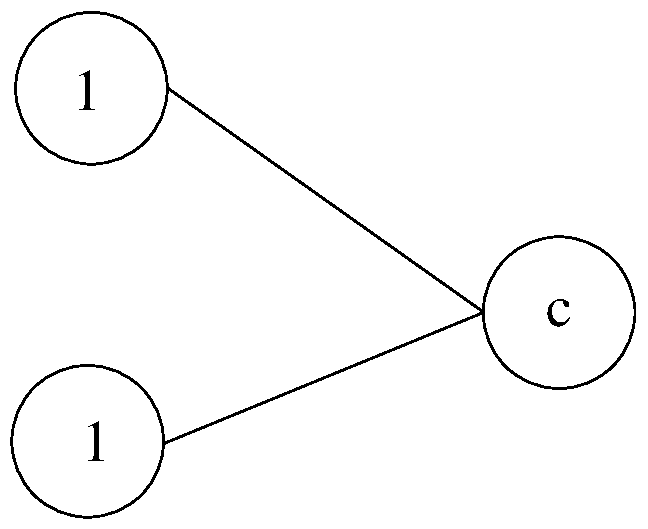
\includegraphics[width=2.5in]{ex2_counter}
	\caption{Counterexample for exercise 2}
	\label{fig:2counter}
\end{figure}

%% -------------------------------------------------------
%%			Exercise 3
%% ------------------------------------------------------

\section*{Exercise 3}
Consider the following approximation algorithm for the cardinality vertex cover problem: Find a depth first search tree $T$ in the given input graph $G$, and return the set $C$ of all the nonleaf vertices of $T$. Show that this is also a 2-approximation algorithm.\\

\textbf{Solution}\\
Let $\mathfrak{D}$ be the Algorithm described above. I assume the Graph $G$ is connected. Otherwise we can find a simple counterexample.

\begin{description}
	\item{\bfseries proposition} The set $C$ returned by $\mathfrak{D}$ is a vertex cover.
	\item{\bfseries proof}

Let $G(V,E)$ be a valid instance for this problem and $T$ the DFS tree generated by $\mathfrak{D}$. A DFS tree in a connected graph visits all nodes. If not, there would exist a edge from a visited node to the unvisited one alongside the algorithm should have taken its path.\\

We now assume, there exists an edge $e=(i,j)\in E$ with $\{i , j\} \cap C = \emptyset$.\\
Every node, as stated above is visited, so $i,j$ may be either nonleaf vertices or leafs of the tree. If either of them would be a nonleaf vertex it would be in $C$. The only left possibility is, that both $i,j$ are leafs.\\
Let $i$ be the vertex visited at first from the DFS Algorithm w.l.o.g.. Then $j$ has to be a child of $i$, because the algorithm expects first all direct childs of $i$ before it returns to the parent of $i$. Because there exist an edge from $i$ to $j$ this edge is either taken in the DFS or there exists an edge from one of $i$ children to $J$. Either way $i$ can't be a leaf.\\

One can conclude, there is no edge, that has no vertex in the set $C$ and that implies, $C$ is a vertex cover.\\
\mbox{} \hfill $\square$  

	\item{\bfseries proposition} $\mathfrak{D}$ is a 2-approximation algorithm.
	\item{\bfseries proof} 

First of all we show, that no leaf is needed to reach an optimal solution.

\end{description}

\label{LastPage}

\end{document}